% !TEX program = xelatex
% index-14.tex
% ref: https://zhuanlan.zhihu.com/p/128341873
% https://www.overleaf.com/learn/latex/Pgfplots_package
\documentclass[UTF8]{article}

\usepackage{pgfplots}
\usepackage{lipsum}
% support cn, default is en
% \usepackage{ctex}

\title{index-14}
\author{oeyoews}
\date{2022/08/12}

\begin{document}
\maketitle

\section{Plots}%
\label{sec:Plots}

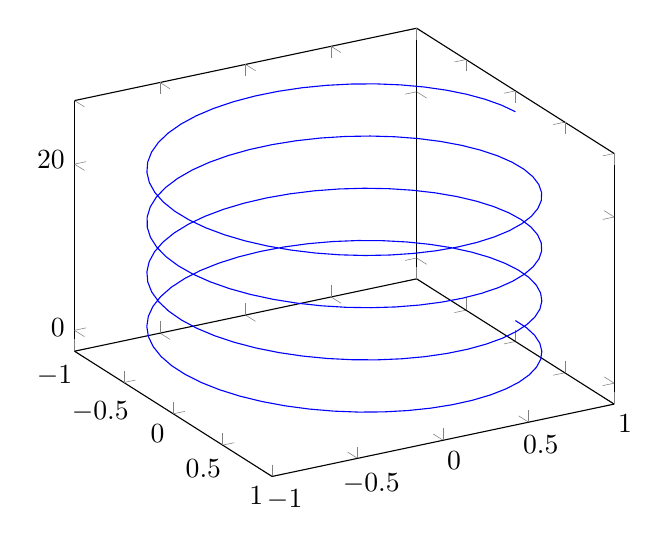
\begin{tikzpicture}
	\begin{axis}
		[
			view={60}{30},
		]
		\addplot3[
			blue,
			domain=0:8*pi,
			samples = 200,
			samples y=0,
		]
		({sin(deg(x))},
		{cos(deg(x))},
		{x});
	\end{axis}
\end{tikzpicture}

%Ex10:3D data plot
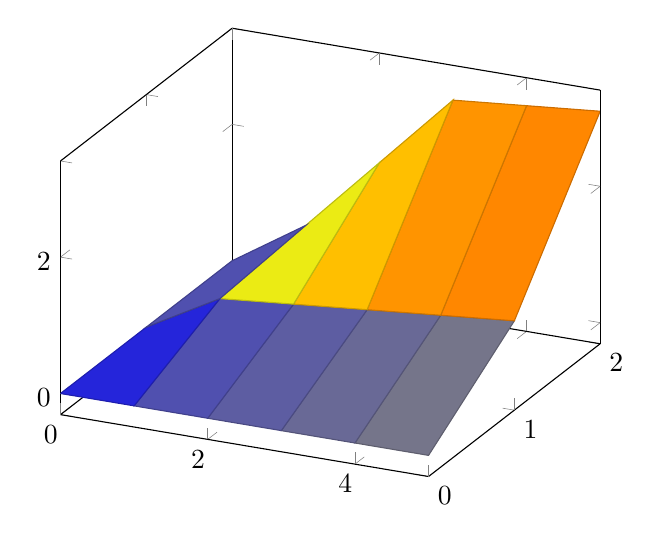
\begin{tikzpicture}
	\begin{axis}
		\addplot3[
			surf,
		]
		coordinates {
				(0,0,0) (0,1,0) (0,2,0)

				(1,0,0) (1,1,0.6) (1,2,0.7)

				(2,0,0) (2,1,0.7) (2,2,1.8)

				(3,0,0) (3,1,0.8) (3,2,2.9)

				(4,0,0) (4,1,0.9) (4,2,3.0)

				(5,0,0) (5,1,1.0) (5,2,3.1)
			};
	\end{axis}
\end{tikzpicture}

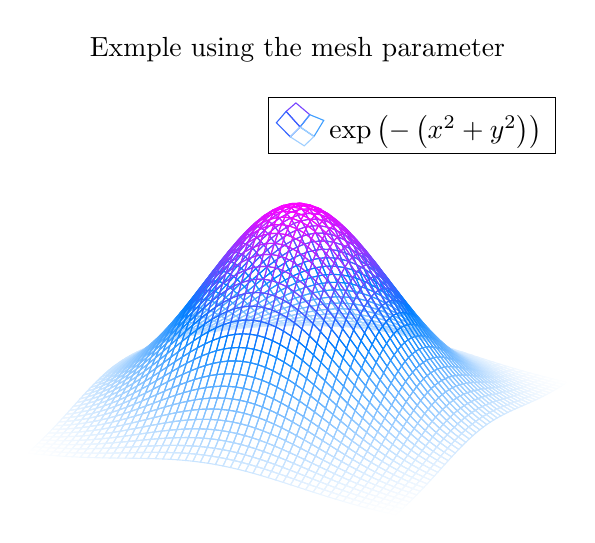
\begin{tikzpicture}
	\begin{axis}[
			title=Exmple using the mesh parameter,
			hide axis,
			colormap/cool
		]
		\addplot3[
			mesh,
			samples=50,
			domain=-1.5:1.5,
		]
		{exp(-(x^2+y^2))};
		\addlegendentry{$\exp\left(-\left(x^2+y^2\right)\right)$}
	\end{axis}
\end{tikzpicture}

%Ex9:3D function
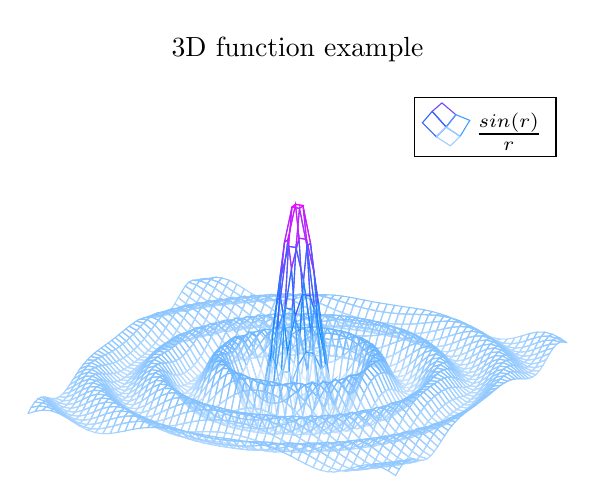
\begin{tikzpicture}
	\begin{axis}[
			title=3D function example,
			hide axis,
			colormap/cool,
		]
		\addplot3[
			mesh,
			samples=50,
			domain=-20:20,
		]
		{sin(deg(sqrt(x^2+y^2)))/sqrt(x^2+y^2)};
		\addlegendentry{$\frac{sin(r)}{r}$}
	\end{axis}
\end{tikzpicture}

\begin{tikzpicture}
	\begin{axis}
		\addplot[color=red]{exp(x)};
	\end{axis}
\end{tikzpicture}

\hskip 10pt

%Here begins the 3d plot
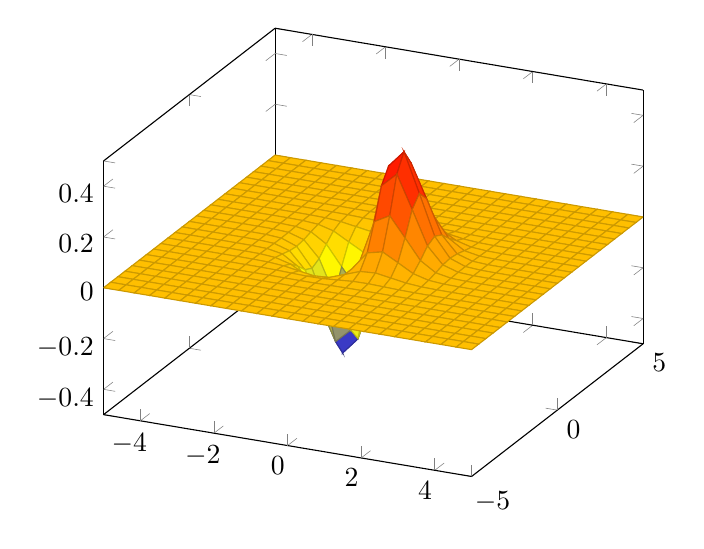
\begin{tikzpicture}
	\begin{axis}
		\addplot3[
			surf,
		]
		{exp(-x^2-y^2)*x};
	\end{axis}
\end{tikzpicture}

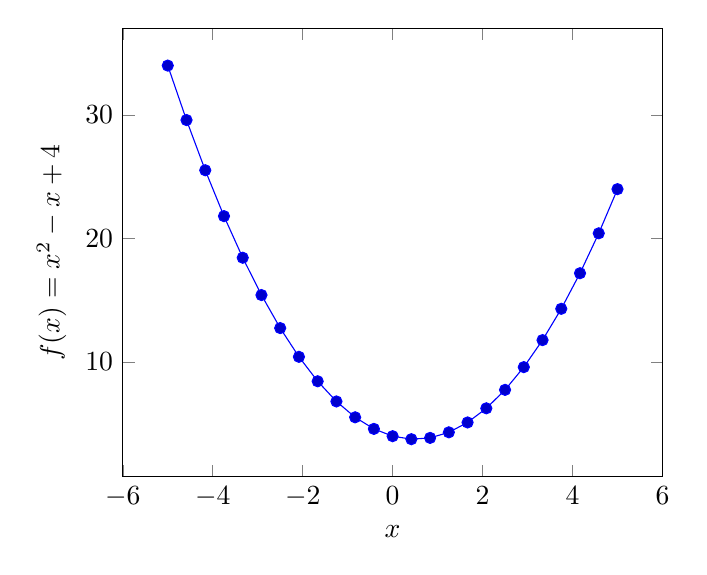
\begin{tikzpicture}
	\begin{axis}[
			xlabel=$x$,
			ylabel={$f(x) = x^2 - x +4$}
		]
		\addplot {x^2 - x +4};
	\end{axis}
\end{tikzpicture}

%Ex4
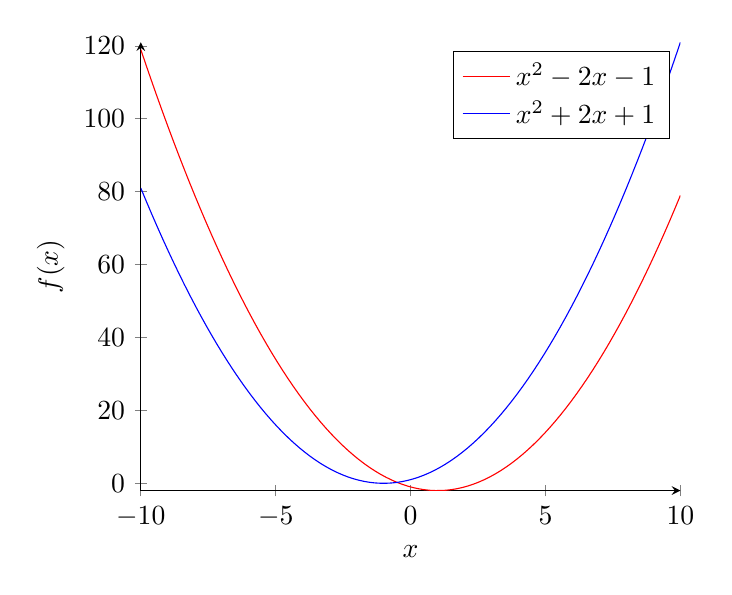
\begin{tikzpicture}
	\begin{axis}[
			axis lines = left,
			xlabel = $x$,
			ylabel = {$f(x)$},
		]
		%Below the red parabola is defined
		\addplot [
			domain=-10:10,
			samples=100,
			color=red,
		]
		{x^2 - 2*x - 1};
		\addlegendentry{$x^2 - 2x - 1$}

		%Here the blue parabloa is defined

		\addplot [
			domain=-10:10,
			samples=100,
			color=blue,
		]
		{x^2 + 2*x + 1};
		\addlegendentry{$x^2 + 2x + 1$}

	\end{axis}
\end{tikzpicture}

%Ex5
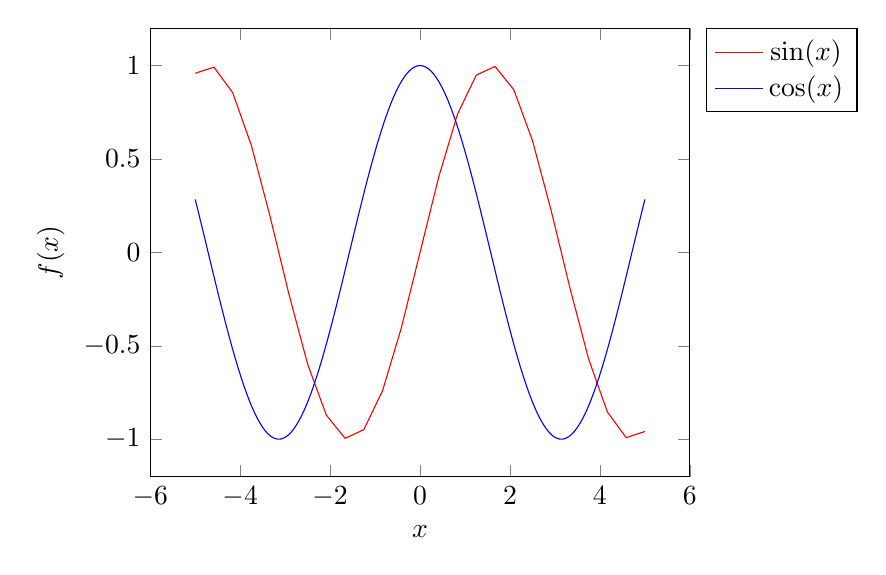
\begin{tikzpicture}
	\begin{axis}[legend pos=outer north east,
			xlabel=$x$,
			ylabel=$f(x)$
		]
		\addplot [red] {sin(deg(x))};
		\addplot [blue,samples=201] {cos(deg(x))};
		\legend{$\sin(x)$,$\cos(x)$}
	\end{axis}
\end{tikzpicture}

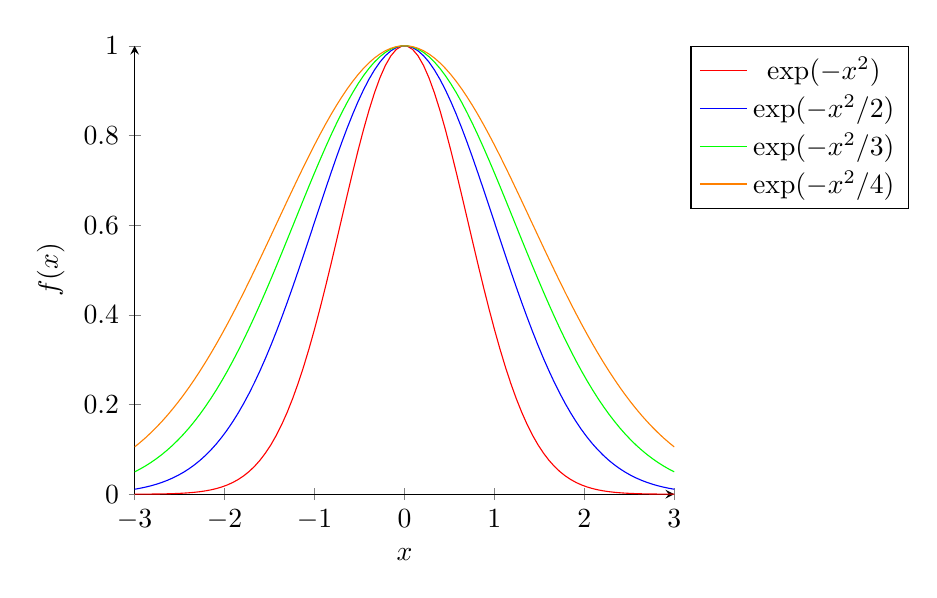
\begin{tikzpicture}
	\begin{axis}[
			legend pos=outer north east,
			axis lines = left,
			xlabel=$x$,
			ylabel=$f(x)$
		]

		\addplot [
			domain=-3:3,
			samples=100,
			color=red,
		]
		{exp(-x^2)};

		\addplot [
			domain=-3:3,
			samples=100,
			color=blue,
		]
		{exp(-x^2/2)};

		\addplot [
			domain=-3:3,
			samples=100,
			color=green,
		]
		{exp(-x^2/3)};

		\addplot [
			domain=-3:3,
			samples=100,
			color=orange,
		]
		{exp(-x^2/4)};

		\legend{$\exp(-x^2)$,
			$\exp(-x^2/2)$,
			$\exp(-x^2/3)$,
			$\exp(-x^2/4)$}

	\end{axis}
\end{tikzpicture}

%Ex6:plot from data
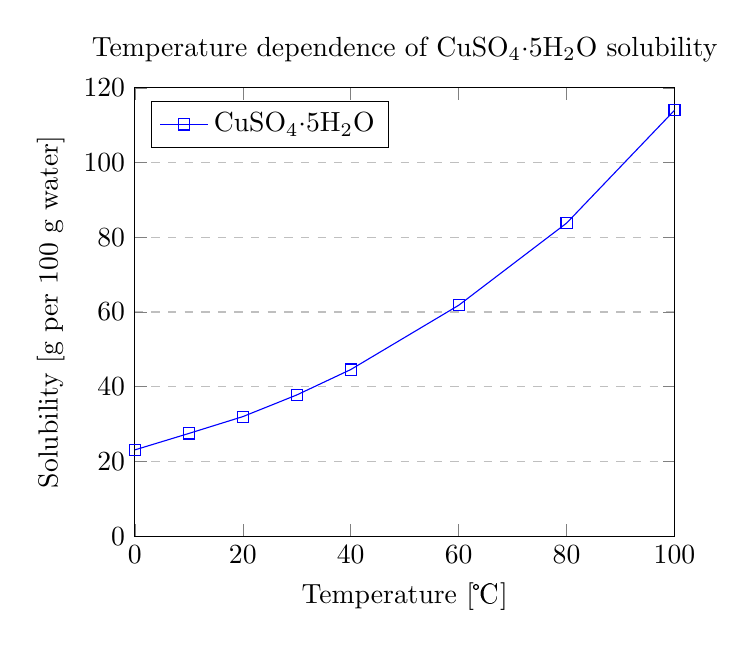
\begin{tikzpicture}
	\begin{axis}[
			title={Temperature dependence of CuSO$_4\cdot$5H$_2$O solubility},
			xlabel={Temperature [\textcelsius]},
			ylabel={Solubility [g per 100 g water]},
			xmin=0, xmax=100,
			ymin=0, ymax=120,
			xtick={0,20,40,60,80,100},
			ytick={0,20,40,60,80,100,120},
			legend pos=north west,
			ymajorgrids=true,
			grid style=dashed,
		]

		\addplot[
			color=blue,
			mark=square,
		]
		coordinates {
				(0,23.1)
				(10,27.5)
				(20,32)
				(30,37.8)
				(40,44.6)
				(60,61.8)
				(80,83.8)
				(100,114)
			};
		\legend{CuSO$_4\cdot$5H$_2$O}

	\end{axis}
\end{tikzpicture}

%Ex7:scatter plots
% \begin{tikzpicture}
% 	\begin{axis}[
% 			enlargelimits=false,
% 		]
% 		\addplot[
% 			only marks,
% 			scatter,
% 			mark=halfcircle*,
% 			mark size=2.9pt]
% 		table[meta=ma] %数据文件中有ma这一列
% 			{scattered_example.dat};
% 	\end{axis}
% \end{tikzpicture}

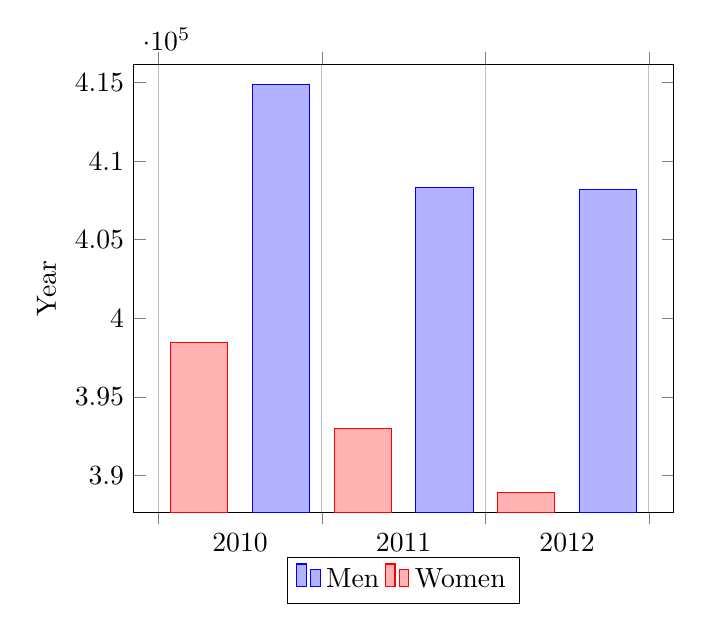
\begin{tikzpicture}
	\begin{axis}[
			x tick label style={/pgf/number format/1000 sep={}},
			ylabel=Year,
			enlargelimits=0.05,
			legend style={at={(0.5,-0.1)},
					anchor=north,legend columns=-1},
			ybar interval=0.7,
		]
		\addplot
		coordinates {(2012,408184) (2011,408348)
				(2010,414870) (2009,412156)};
		\addplot
		coordinates {(2012,388950) (2011,393007)
				(2010,398449) (2009,395972)};
		\legend{Men,Women}
	\end{axis}
\end{tikzpicture}
\end{document}
